\documentclass[journal,12pt,twocolumn]{IEEEtran}
\usepackage{hyperref}
\usepackage{graphicx}
\usepackage{amsmath}
\title{Assignment 1}
\author{JARPULA BHANU PRASAD - AI21BTECH11015	}
\date{April 2021}
\begin{document}
\maketitle
\Large \underline{Download codes from}:\\
\large Python code for graph - \href{https://github.com/jarpula-Bhanu/Assinment-1/blob/main/quardratic.py}{python}.\\And c-code for roots -  \href{https://github.com/jarpula-Bhanu/Assinment-1/blob/main/roots.c}{c-code}.\\And latex code from - \href{https://github.com/jarpula-Bhanu/Assinment-1/blob/main/Assignment_1.tex}{Latex}.

\section{\Large \underline{Problem-ICSE-2019-10  Q)4-b}}
\large \noindent Q)Solve for $x$ the quadratic equation $$x^2-4x-8=0.$$ Give your answer correct to three significant figures.
\section{\large \underline{solution}}
Given quadratic equation,
\begin{align} \label{1}
\large x^2-4x-8=0.
\end{align}

\noindent Solution for the quadratic equation is the form 
\begin{align} \label{2}
 \large ax^2+bx+c=0.
\end{align} 
 is given by 
\begin{align} \label{3}
\framebox[1.1\width]{\LARGE $\frac{-b\pm\sqrt{b^2-4ac}}{2a}$}
\end{align}

let $\alpha$ and $\beta$ be the roots of the equation,\\Such that,
\begin{align} \label{4}
\framebox[1.1\width]{$\alpha$ =\Large $\frac{-b+\sqrt{b^2-4ac}}{2a}$ and  $\beta$ =\Large $\frac{-b-\sqrt{b^2-4ac}}{2a}$}
\end{align}

Now, on comparing the coefficients from 
\\eqn\eqref{1} and eqn\eqref{2}.
\\\large $a$=1,\large $b$=-4 and \large $c$=-8.
\\Substituting values in eqn\eqref{4}. we get,
\begin{align} \label{5}
\alpha =\Large \frac{-(-4)+\sqrt{(-4)^2-4(1)(-8)}}{2(1)}
\end{align}

and

\begin{align} \label{6}
\beta =\Large \frac{-(-4)-\sqrt{(-4)^2-4(1)(-8)}}{2(1)}
\end{align}

On simplifying \eqref{5} and \eqref{6} we get,
\begin{align}
\alpha=2+2\sqrt{3}  \\ \beta=2-2\sqrt{3} 
\end{align}
i.e., The roots of the equation are,
\begin{align}
\alpha=5.464   \\ \beta=-1.464
\end{align}
On rounding off to three significant figures.
\\The roots of the equation are,
\begin{align} 
\framebox[1.1\width]{$\alpha$=5.46 and $\beta$=-1.46.}
\end{align}
\begin{figure}[h] 
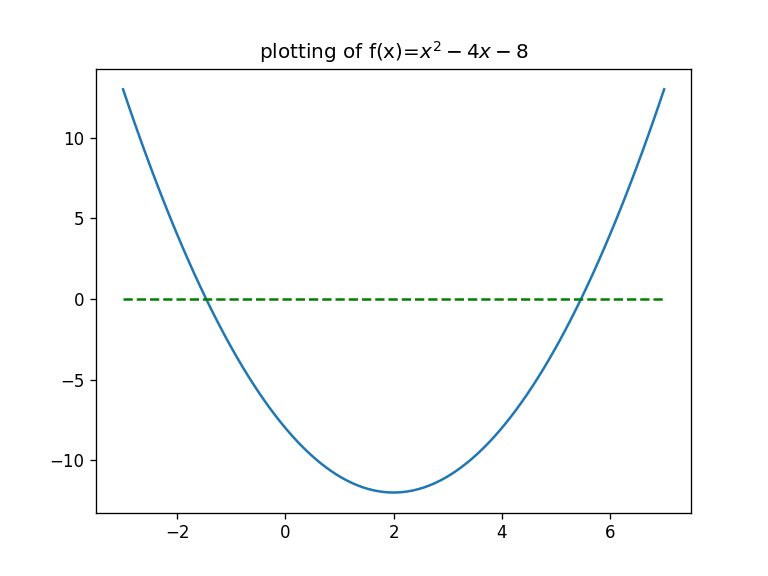
\includegraphics[scale=0.65] 
{Figure_0}\large
\caption{graph 1:Roots of the equation}
\label{fig:a}
\end{figure}

\noindent The above graph \pageref{fig:a}   gives the roots of the equation 

\end{document}
